% !TeX spellcheck = IT
\documentclass[12pt]{article}
\usepackage[top=1.5in, bottom=1.5in, left=1in, right=1in]{geometry}
\usepackage[utf8]{inputenc}
\usepackage[italian]{babel}
\usepackage{graphicx}
\usepackage{caption}
\usepackage[colorlinks=false,linkcolor=blue]{hyperref}
\usepackage{nameref} 
\graphicspath{{./images/}}
\def\code#1{\texttt{#1}}
\def\image[#1][#2]#3{
  \begin{figure}[h]
  \centering
  \includegraphics[#2]{#1}
  \caption{#3}
  \end{figure}}
\def\boximage[#1][#2]#3{
	\begin{figure}[h]
		\centering
		\fbox{
		\includegraphics[#2]{#1}}
		\caption{#3}
\end{figure}}
\title{Il database sottostante Git}
\author{Arianna Masciolini}

\begin{document}
\maketitle
\newpage
\tableofcontents
\newpage
\section{Introduzione}
Un \textit{Version Control System} (VCS) è un sistema che tiene traccia delle modifiche apportate ad uno o più file in modo da garantire all'utente la possibilità di accedere alle versioni precedenti dei file suddetti in qualsiasi momento. 
\bigskip \\
I primi sistemi di controllo di versione, locali, nacquero con l'idea di risolvere i problemi legati a quello che potrebbe essere definito versioning "manuale", consistente nel conservare più copie dei file d'interesse: la forte suscettibilità a errori e lo spreco di spazio su disco. Tra questi VCS locali, RCS ha goduto ha lungo di grande popolarità: esso salva su disco, in un particolare formato, una serie di \textit{patch}, ossia le differenze tra una versione e l'altra dei file, in modo tale da poter ricostruire lo stato in cui era ognuno di essi in qualsiasi momento, applicandovi una dopo l'altra le varie patch.
\bigskip \\
Successivamente, ci si pose il problema di permettere a più persone di collaborare a distanza. Per risolverlo nacquero i sistemi centralizzati di controllo di versione (CVCS), come CVS, Subversion, e Perforce. In questi sistemi, per il resto analoghi ad RCS e simili, tutte le versioni dei file controllati sono salvate su un unico server e rese così disponibili ai diversi utenti. Anche questo approccio presenta però problematiche importanti, dovute al fatto che il server centrale rappresenta un punto di vulnerabilità per l'intero sistema. 
\bigskip \\
I DVCS (\textit{Distributed VCS}), di cui Git, Mercurial, Bazaar e Darcs sono gli esempi più noti, risolvono questo problema: i membri del gruppo non si limitano a scaricare la più recente versione dei file, ma copiano l'intero repository, cosicchè ogni client costituisce un backup completo del progetto.
\begin{figure}[h]
	\centering
		\begin{minipage}{4cm}
			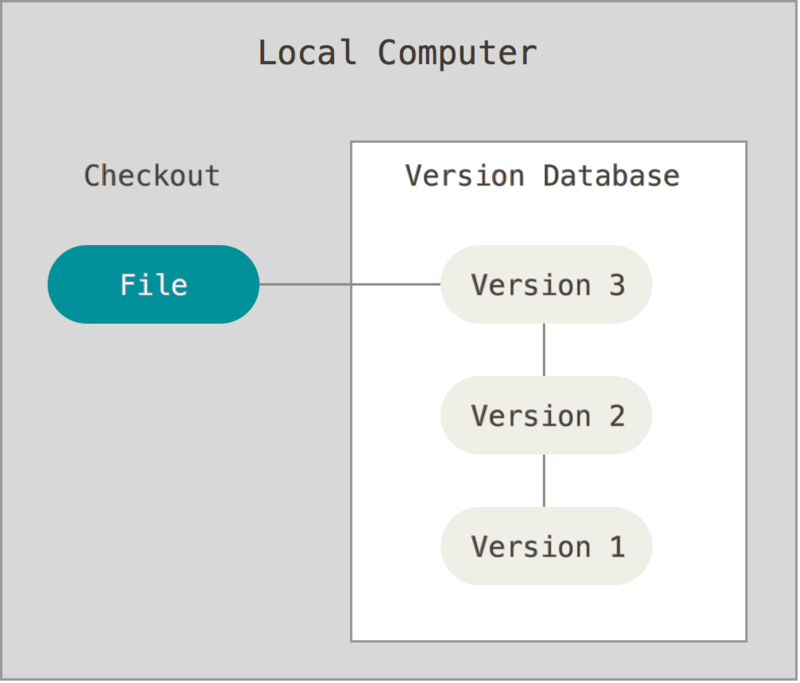
\includegraphics[height=3.5cm]{local.png}
		\end{minipage}
		\qquad
		\begin{minipage}{4cm}
			 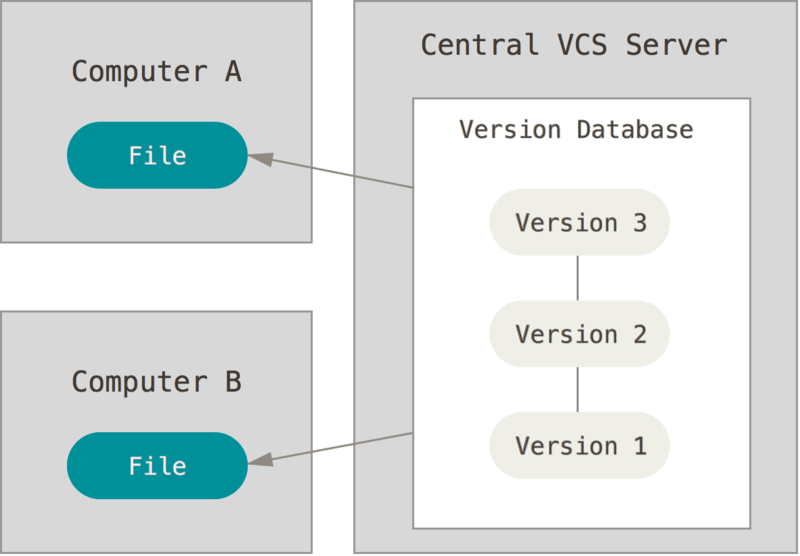
\includegraphics[height=3.5cm]{centralized.png}
		\end{minipage}
		\qquad
		\qquad
		\begin{minipage}{4cm}
			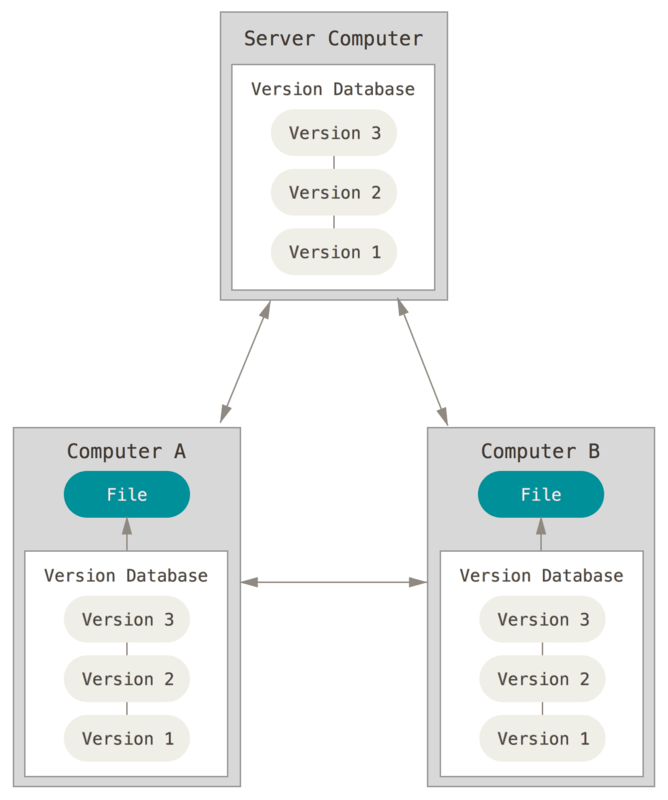
\includegraphics[height=3.5cm]{distributed.png}
		\end{minipage}
	\caption{Confronto tra un VCS locale, un CVCS e un DVCS.}
\end{figure}
\\In particolare, Git -ad oggi il VCS più diffuso \cite{openhub}- si differenzia tanto dagli altri sistemi distribuiti quanto dai loro predecessori per il modo in cui memorizza i dati: non come una serie di \textit{patch} legate ai vari file, ma come una serie di "istantanee" di un filesystem in miniatura, accessibili tramite puntatori.
L'obiettivo di questa relazione è, per l'appunto, descrivere l'approccio adottato da Git in tale ambito, in modo da comprendere quali ne siano i vantaggi rispetto alle soluzioni adottate dai sistemi concorrenti.
Nella sezione successiva verranno brevemente richiamati alcuni concetti di base riguardo il funzionamento di Git, utili per rendere più chiare e sintetiche le spiegazioni più strettamente legate al suo modello di branching e al sottostante database.  
\section{Nozioni di base su Git}
Git, nato nel 2005 per favorire lo sviluppo del kernel Linux, è un sistema di controllo versione completamente distribuito che deve il suo successo al proprio modello di branching, che lo rende ottimale per la gestione di progetti open source, che hanno quasi sempre uno sviluppo non lineare.
\bigskip \\
Come si è accennato nella sezione precedente, Git adotta un approccio radicalmente differente rispetto a quello tradizionale, il cosiddetto controllo versione \textit{delta-based}, basato su una lista di \textit{patch}, ossia di modifiche, legate ai singoli file. Un repository Git è infatti una sorta di filesystem Unix-like semplificato, di cui viene fatta una sorta di "istantanea" resa accessibile mediante un puntatore ogniqualvolta lo stato del progetto viene salvato.
\begin{figure}[h]
	\centering
	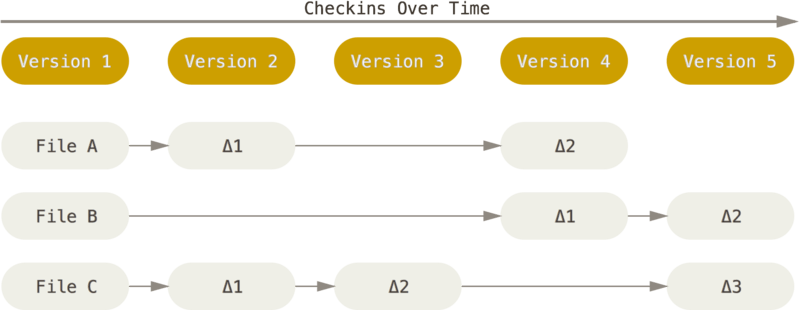
\includegraphics[width=13cm]{delta-based.png}
	\caption*{(a)\bigskip}
	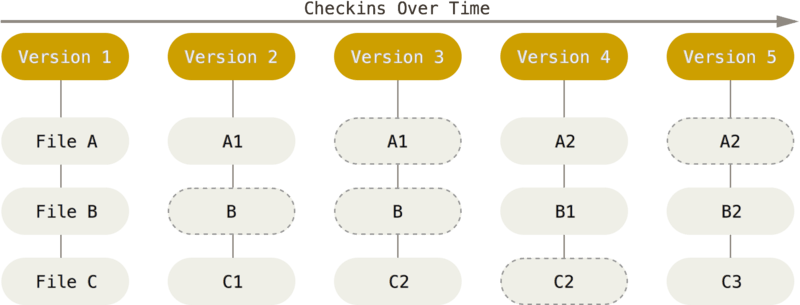
\includegraphics[width=13cm]{snapshots-based.png}
	\caption*{(b)}
	\caption{Confronto il modo in cui vengono salvati i dati in un VCS delta-based (a) e quanto avviene in Git (b).}
\end{figure}
\bigskip \\
Quasi tutte le azioni possibili in Git consistono, in ultima analisi, nell' \textit{aggiungere} dati al sottostante database. Cancellare dei dati e, in generale, compiere azioni distruttive, è reso volutamente difficile, in modo tale da rendere pressoché impossibile perdere il proprio lavoro, se non altro a seguito di un \textit{commit}, l'azione tramite la quale i cambiamenti al repository vengono salvati.
\bigskip \\
Per meglio comprendere quale sia il significato di un commit in Git e, in generale, per ottenere un buon modello concettuale del funzionamento di tale sistema di controllo versione, è fondamentale conoscere gli stati in cui può trovarsi un file all'interno di un repository:
\begin{itemize}
	\item \textit{modified}: sono state effettuate delle modifiche al file, non ancora confermate tramite un commit;
	\item \textit{staged}: il file, che ha subito delle modifiche, è stato marcato come parte del prossimo commit;
	\item \textit{committed}: il file è salvato permanentemente nel database locale tramite, appunto, un commit.
\end{itemize}
A questo punto è opportuno parlare della struttura di un repository Git, le cui parti principali sono:
\begin{itemize}
	\item il \textit{working tree}, consistente in una copia di una specifica versione del progetto, estratta dal database in modo da poter essere modificata dall'utente;
	\item la cartella \code{.git}, dove vengono si trovano i metadati e l'\textit{object database}, sui cui ci soffermerà nella prossima sezione, relativi al progetto;
	\item la \textit{staging area}, ossia un file (generalmente contenuto nella cartella \code{.git}) contenente le informazioni relative al contenuto del prossimo commit.
\end{itemize}
E' facile intuire, a questo punto, quale sia il tipico modo di procedere quando si lavora ad un progetto gestito con Git: dopo aver modificato uno o più file nel \textit{working tree}, si selezionano le modifiche di cui tener traccia nel commit successivo, aggiungendoli così alla \textit{staging area}. Nel momento in cui viene eseguito il comando \code{git commit} lo stato dei file nella \textit{staging area} viene salvato nella cartella \code{.git}.
\paragraph{Checksumming}
Un'ulteriore, importante funzionalità di Git, parte integrante della sua filosofia, è quella di verificare qualsiasi file o directory, prima di archiviarlo, tramite una checksum che è poi utilizzata per riferirvisi. Ciò significa che è impossibile cambiarne il contenuto senza che Git ne sia a conoscenza, il che permette di rilevare qualsiasi perdita o corruzione di dati in transito. 
Il meccanismo impiegato per generare tale checksum è la funzione crittografica SHA-1, il cui output, basato sul contenuto di un file o sulla struttura interna di una cartella, è un numero esadecimale di 40 caratteri.
\image[init_tree.png][width=9.5cm]{La struttura del repository \code{demo}, appena creato con il comando \code{git init}.}
\section{Il database di Git} % chapter: Git internals -> Git objects
%Git può essere definito come \textit{\underline{filesystem} orientato ai contenuti}. Questo significa che il nucleo di Git è un database chiave-valore: all'inserimento di un oggetto in un \underline{repository}, Git restituirà la \underline{chiave} con la quale esso è univocamente identificato. Per meglio rendersi conto del funzionamento di tale database, è opportuno inizializzare un repository

\newpage
\begin{thebibliography}{9}
	\bibitem{git_pro}
	Scott Chacon, Ben Straub. \textit{Git Pro}, seconda edizione, 2014.
	\bibitem{openhub}
	\url{openhub.net}
\end{thebibliography}
\end{document}